% ==================================================
%
%   模型的建立与求解
%
% --------------------------------------------------

\section{模型的建立与求解}

\begin{figure}[h]
    \centering
    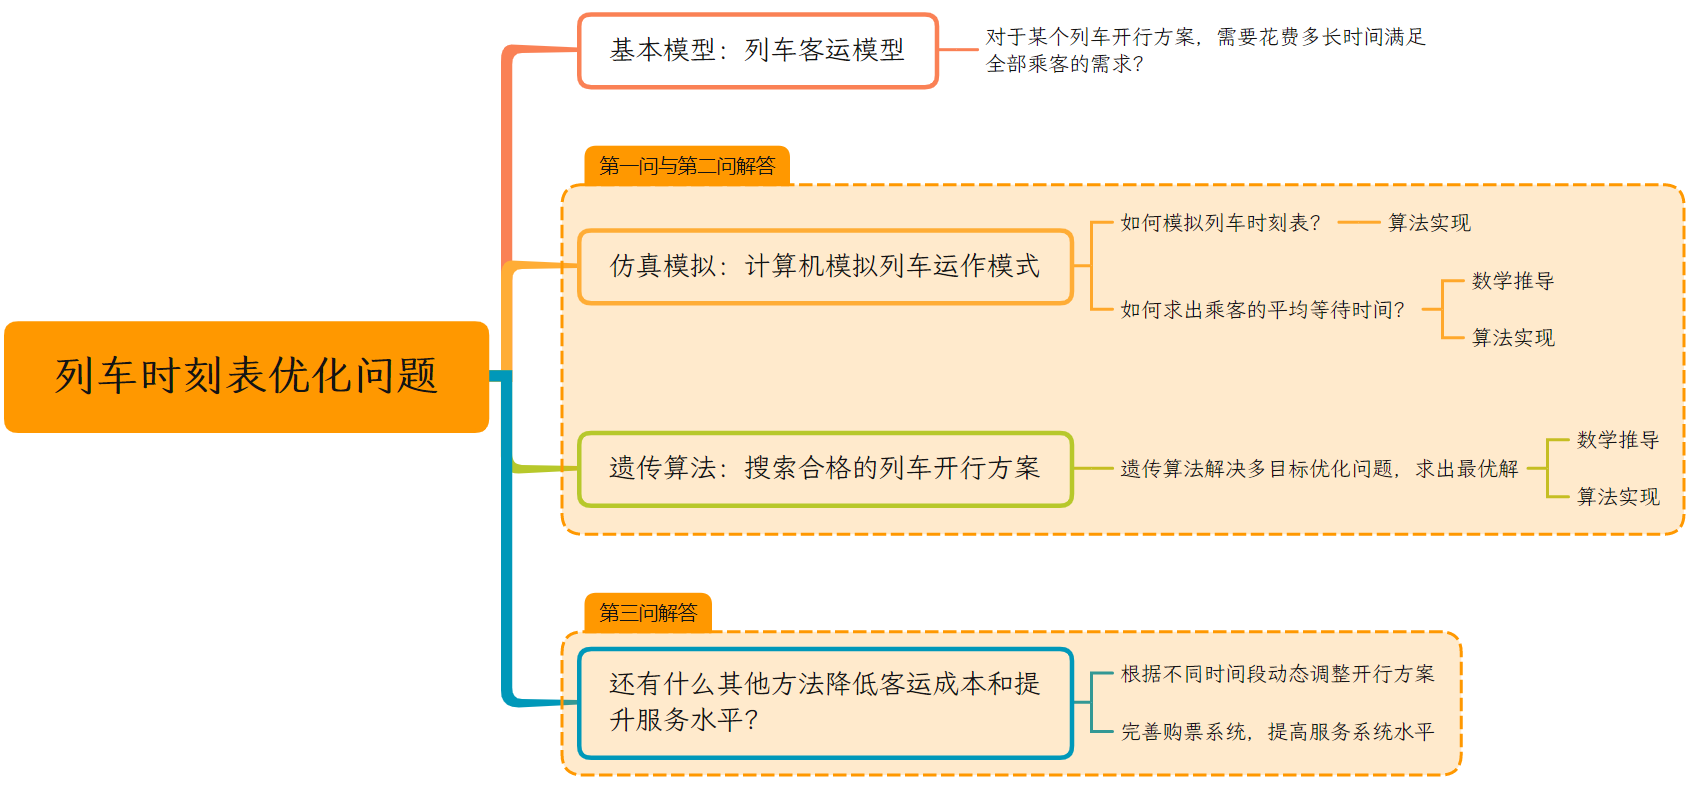
\includegraphics[scale=0.2]{res/figure161100.png}
    \caption{模型思维图}
\end{figure}

% ............ 模型的准备 ............ %

\subsection{模型的准备}

为了方便后续对问题的分析和建立,这里先给出\textbf{列车客运模型}与\textbf{遗传算法}的概述,旨在方便读者更好的理解解题模型的核心思想。

\subsubsection{列车客运模型}

列车客运模型是一种简化的列车运行模型。

为了方便表述,考虑只有$5$个车站的情况。在这$5$个车站中,从前到后依次标号为$1-5$。设发车的间隔时间为$\Delta t$,那么在该开行方案下,需要耗费多长时间才能满足所有乘客的需求?

利用列车行程图,可以清晰的展现出列车的运行模式。

\begin{figure}[h]
    \centering
    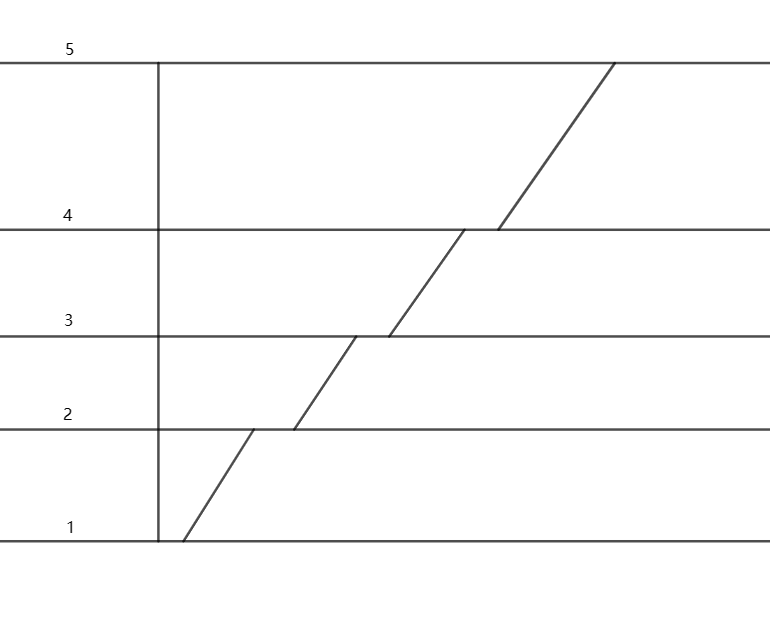
\includegraphics[scale=0.3]{res/figure160314.png}
    \caption{列车运行图}
\end{figure}

考虑现实情况以及OD客流数据,每趟列车上车的乘客是按照乘客需求的比例分配的。例如,在车站$1$时,某一次的上车乘客比例于OD客流数据比例相等。但是伴随着后面的列车的运行过程,因为下车的乘客数量是不一定的所以说,下车的时间是不一定的。为了考虑这样的情况,我们必须要给出很多合理的解释。这是因为原本在这个车站下车的人数就有所变化,对于这种非数值计算类问题,在文后将尝试采用程序模拟的办法的最后的运行结果,而求出我们最开始给出的问题——需要耗费多长时间才能满足所有乘客的需求?

该模型主要功能是描述列车的运行模式,为接下来的仿真模型做出准备。

\subsubsection{遗传算法简介}

遗传算法(Genetic Algorithm, GA)也被称为进化算法(Evolutionary Algorithm)。该算法是一种仿生算法,旨在通过模仿生物遗传演化机制,达到优化群落的目的\cite{hanJiyuyichuanheshengsuanfaqiujiehanshuyouhuawenti2010}。为了更好的理解遗传算法,让我们回顾一下自然界中生物的演化是如何进行的?

生物学表明,生物的演化是以种群为单位的,而演化的本质是基因的变异。

还有个更重要的东西——自然选择。或者通俗的理解为,种群对环境的适应度。宏观上看的话,种群是朝着适应度高的方向进行的。

根据以上论述,可以提炼出遗传算法的三个要素:

\begin{enumerate}
    \item 种群——基因与染色体
    \item 演化
    \item 适应度
\end{enumerate}

在遗传算法中,首先可以根据随机数算法生成初始群落。紧接着使该种群中的个体相互交配繁衍,产生新的个体。在产生新的个体的过程中,要确保完成两个操作:染色体的交叉互换和基因变异。前者保证优秀的基因有可能配对在一起,后者保证了种群的基因多样性,防止种群的基因趋同,这样可以防止算法陷入局部最优解。产生了下一代以后,接下来计算出所有个体的适应度,剔除适应度最低的那几些个体,使得产生个体数量与初始群落一致的第二代群落。最后一次遗传算法的迭代就已经完成(如图\ref{GeneticAlgorithmDiagram})。

设定遗传算法迭代的终止,最后得到的种群就是最优解集,可以取最高适应度作为最终的解。

\begin{figure}[h]
    \centering
    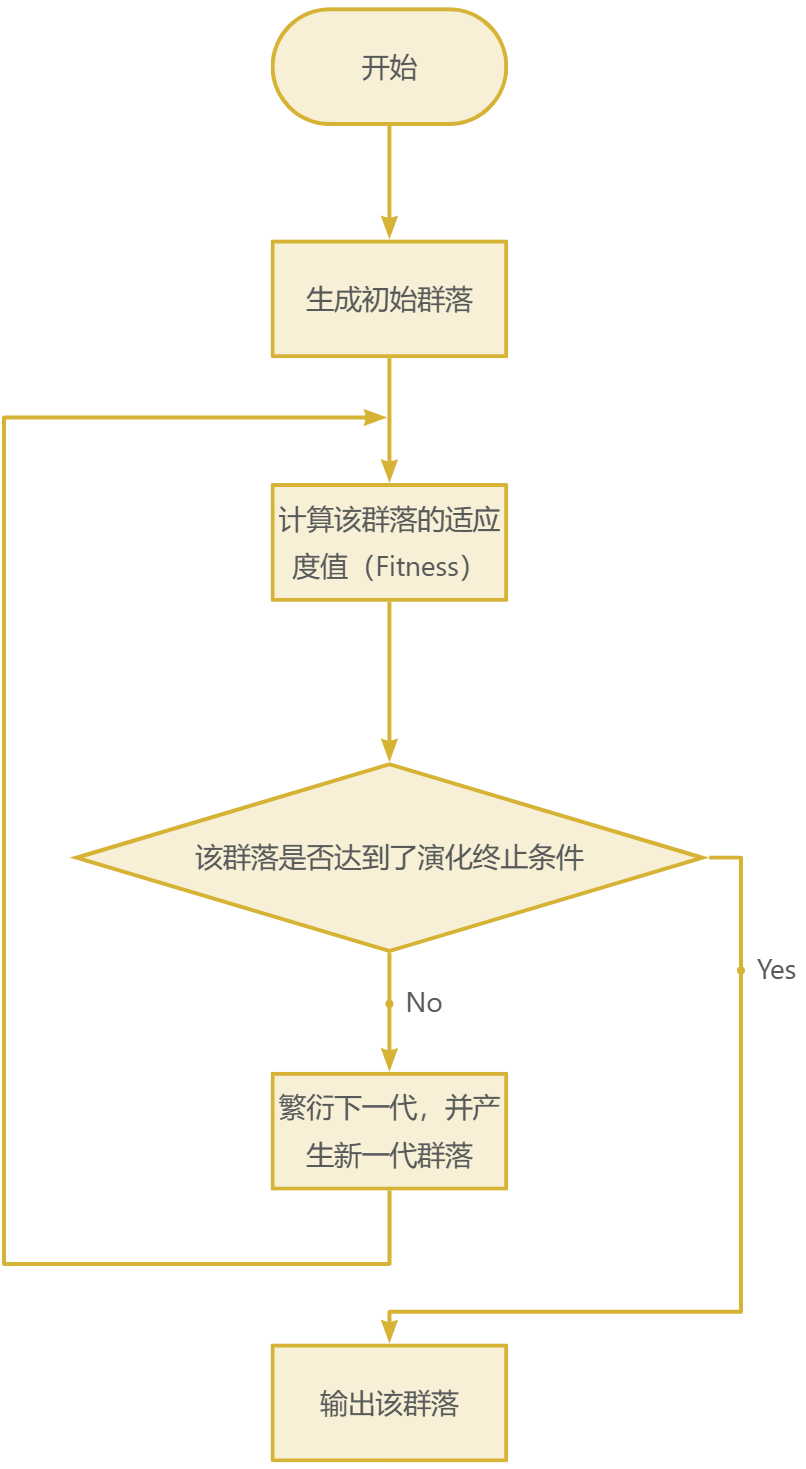
\includegraphics[scale=0.15]{res/GeneticAlgorithmDiagram.png}
    \caption{遗传算法框图}
    \label{GeneticAlgorithmDiagram}
\end{figure}

实际上,遗传算法最大的难点在于演化这一步骤。在一般算法中,演化有两个重要操作需要进行——基因互换和染色体的变异,可以说,对这两个操作的设计涵盖了整个遗传算法的绝大部分设计。


% ............ 模型的准备 ............ %

\subsection{问题$1$模型的建立与求解}

\subsubsection{仿真模拟计算:计算机模拟列车的运作模式}

为了求出相关的计算方法

\subsubsection{动态规划求解列车客运模型}

\subsubsection{和声遗传算法搜寻帕累托最优解}

% ............ 模型的准备 ............ %

\subsection{问题二}

\subsubsection{}

\subsection{问题三:针对不同时间段动态调整列车开行方案}

事实上,节假日的旅游乘客会比工作日的旅游乘客多。从中华人民共和国交通运输部公布的数据可以看出来,在2023的1-2月份的旅客明显增加\cite{ChengShiKeYunTongJiShuJuZhongHuaRenMinGongHeGuoJiaoTongYunShuBu}。一方面是因为日近春节,人们需要回家,另一方面疫情放开,在家中憋了很多时间的人也逐渐开始旅游,回归正常生活。

所以为了应对这样的情况,应该针对不同时间段动态地调整列车开行方案,提高列车服务质量。

然而,影响列车运营成本的两个根本因素是客流数据和计算过程就

\subsubsection{背景}


% ==================================================
%
%   模型的评价与改进
%
% --------------------------------------------------

\section{模型的评价与改进}

